\documentclass[a4paper]{article}

%% Language and font encodings
\usepackage[utf8]{inputenc}
\usepackage[italian]{babel}
\usepackage[T1]{fontenc}
\usepackage{multicol}
\usepackage{enumerate}
\usepackage[normalem]{ulem}
\useunder{\uline}{\ul}{}
\usepackage{multirow}
\usepackage{tabularx}
\usepackage[bottom]{footmisc}
\usepackage{wrapfig}
\usepackage[table]{xcolor}
\usepackage{float}
\usepackage[font=small,labelfont=bf]{caption}
\usepackage{url}
\usepackage{subcaption}
\usepackage{chngcntr}
\usepackage{amssymb}
\newcounter{rowno}
\counterwithin{figure}{section}
\counterwithin{table}{section}

\let\oldtexttt\texttt
\let\texttt\path


\definecolor{grigio_chiaro}{gray}{0.95}

%% Sets page size and margins
\usepackage[a4paper,
top=1.5cm,
bottom=1.5cm,
left=1.5cm,
right=1.5cm,
marginparwidth=1.75cm]{geometry}

%% Useful packages
\usepackage{amsmath}
\usepackage{graphicx}
\usepackage[colorinlistoftodos]{todonotes}
\usepackage[colorlinks=true, allcolors=blue]{hyperref}

\title{Human Resources Analytics \\ Data Mining, A.A. 2017/2018}


\author{Carlo Alessi \\ Francesco Cariaggi \\ Leonardo Cariaggi}

\begin{document}
\maketitle
\date{}

\tableofcontents

\newpage

\section{Data understanding}

In questa sezione si illustra il processo di \textit{data understanding} attuato sul dataset. In particolare, nel paragrafo 1.1 si descrive la semantica e il tipo dei dati. Nel paragrafo 1.2 si discute la distribuzione degli attributi e si presentano alcune statistiche. Nel paragrafo 1.3 si valuta la qualità dei dati (rilevazione dei valori mancanti e degli \textit{outlier}). Nel paragrafo 1.4 si descrivono quindi le trasformazioni applicate ai valori degli attributi. Infine, nel paragrafo 1.5, si ragiona sulla correlazione tra coppie di attributi e sull'eventuale eliminazione di attributi ridondanti (in base ai risultati ottenuti).

\subsection{Semantica dei dati}

Ogni riga del dataset contiene le informazioni di un singolo impiegato dell'azienda. La tabella \ref{tab:semantics} mostra la semantica e il tipo del valore di ogni colonna del dataset:

\begin{table}[h]
\centering


\begingroup
\setlength{\tabcolsep}{8pt} % Default value: 6pt
\renewcommand{\arraystretch}{1.4} % Default value: 1
\rowcolors{1}{grigio_chiaro}{white}
\begin{tabularx}{\textwidth}{|lXlX|}
\hline
\textbf{Nome dell'attributo} & \textbf{Descrizione}                                                              & \textbf{Tipo} & Dominio\\\hline
satisfaction\_level          & Livello di soddisfazione dell'impiegato  & Numerico, continuo  & ${[}0,1{]}\subseteq\mathbb{R}$  \\ 
last\_evaluation             & Ultima valutazione delle performance dell'impiegato                                   & Numerico, continuo  & ${[}0,1{]}\subseteq\mathbb{R}$\\ 
number\_project              & Numero di progetti completati dall'impiegato nel periodo di lavoro                               & Numerico, discreto  & $\mathbb{N^+}$  \\ 
average\_montly\_hours       & Numero medio di ore trascorse dall'impiegato ogni mese sul posto di lavoro                       & Numerico, discreto   & $\mathbb{N^+}$   \\ 
time\_spend\_company         & Numero di anni trascorsi dall'impiegato nell'azienda                                             & Numerico, discreto   & $\mathbb{N^+}$   \\ 
Work\_accident               & Indica se l'impiegato ha avuto un incidente sul posto di lavoro o meno                                         & Numerico, categorico   & $ \{ 0, 1 \}$   \\ 
left                         & Indica se l'impiegato ha lasciato il posto di lavoro o meno                       & Numerico, categorico   & $ \{ 0, 1 \}$   \\ 
promotion\_last\_5years      & Indica se l'impiegato ha ottenuto una promozione negli ultimi 5 anni o meno     & Numerico, categorico   & $ \{ 0, 1 \}$   \\ 
sales                        & Dipartimento per il quale l'impiegato lavora                                      & Stringa, non ordinale   & $ \{'sales','accounting',$\newline
$'hr','technical',$\newline
$'support','management',$\newline
$'IT','product_mng',$\newline
$'marketing','RandD'\}$    \\ 
salary                       & Fascia di salario nella quale rientra l'impiegato     & Stringa, ordinale    & $ \{ 'low', 'medium', 'high' \}$   \\ \hline
\end{tabularx}
\endgroup
\caption{Semantica dei dati}
\label{tab:semantics}
\end{table}

\subsection{Distribuzione degli attributi e statistiche}

\noindent La tabella \ref{tab:statistics} mostra invece alcune statistiche riguardanti i valori degli attributi nel dataset: per ogni variabile sono riportate, in ordine, il numero di record per cui il valore non è mancante, la media, la deviazione standard, il minimo, i quartili (primo, secondo e terzo) e infine il massimo. Gli attributi booleani sono stati inclusi solo per avere un'idea della frequenza dei diversi valori in punti percentuali.

\begin{table}[h]
\centering

\setlength{\tabcolsep}{6pt} % Default value: 6pt
\renewcommand{\arraystretch}{1.3} % Default value: 1
\rowcolors{1}{grigio_chiaro}{white}

\begin{tabularx}{\textwidth}{|XXXXXXXXX|}
\hline
      & satisfaction level & last evaluation & number project & average montly hours & time spend company & Work accident & left    & promotion last 5years \\
count & 14999             & 14999          & 14999         & 14999                & 14999              & 14999        & 14999 & 14999                 \\
mean  & 0.613               & 0.716            & 3.803           & 201.05                 & 3.498                & 0.145          & 0.238   & 0.021                   \\
std   & 0.249               & 0.171            & 1.233           & 49.943                 & 1.46                 & 0.352          & 0.426   & 0.144                   \\
min   & 0.09                & 0.36             & 2             & 96                   & 2                  & 0            & 0     & 0                     \\
25\%  & 0.44                & 0.56             & 3             & 156.0                  & 3                  & 0            & 0     & 0                     \\
50\%  & 0.64                & 0.72             & 4             & 200.0                  & 3                  & 0            & 0     & 0                     \\
75\%  & 0.82                & 0.87             & 5             & 245.0                  & 4                  & 0            & 0     & 0                     \\
max   & 1.0                 & 1.0              & 7             & 310                  & 10                 & 1            & 1     & 1       \\ \hline       
\end{tabularx}
\caption{Statistiche del dataset}
\label{tab:statistics}
\end{table}

\noindent Di seguito si mostrano, separatamente, le distribuzioni degli attributi categorici e numerali del dataset. Precisamente, la figura \ref{fig:distrib_categ} mostra la distribuzione degli attributi categorici: nell'asse delle ascisse sono riportati i valori assunti da ogni variabile, mentre sulle ordinate compare la frequenza dei singoli valori.

\noindent
\begin{center}
 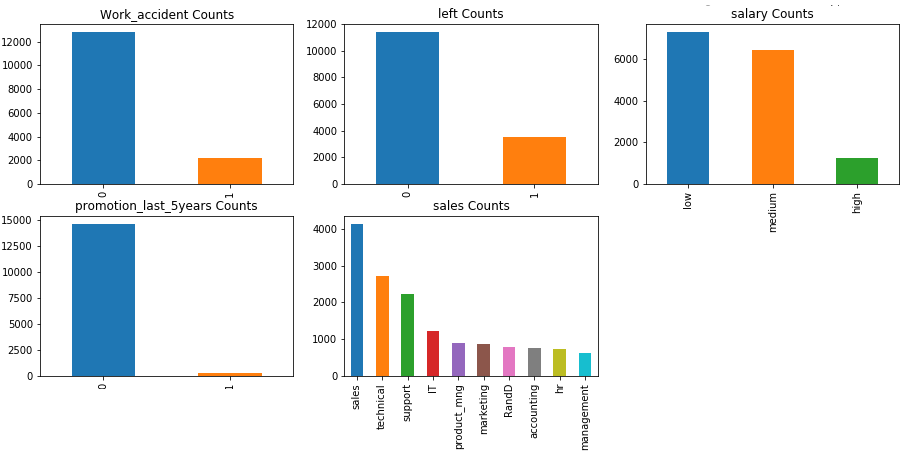
\includegraphics[width=0.85\textwidth]{distribution_categoricals_large.png}
 \captionof{figure}{Distribuzione delle variabili categoriche}
 \label{fig:distrib_categ}
\end{center}

\noindent La figura \ref{fig:distrib_numer}, invece, riporta gli istogrammi che riassumono la distribuzione delle variabili numeriche del dataset. Le feature \texttt{number_project} e \texttt{time_spend_company}, in questa sezione, sono considerate numeriche (sebbene in altre fasi dell'analisi esse assumano il ruolo di variabili categoriche).

\noindent
\begin{center}
 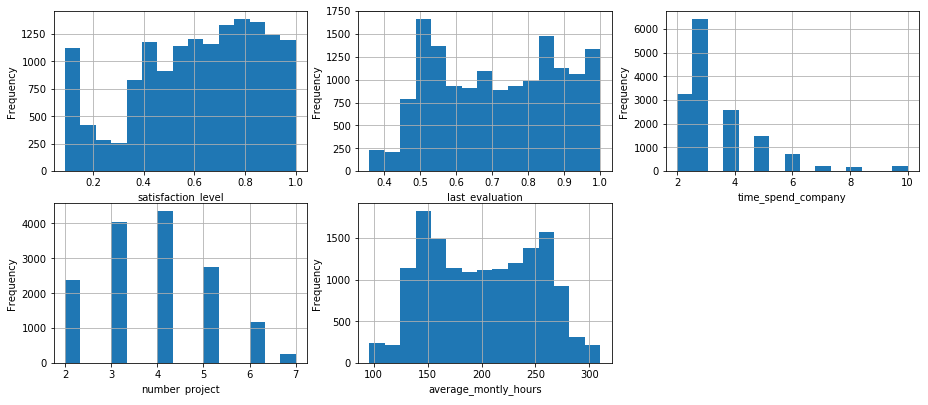
\includegraphics[width=0.9\textwidth]{distribution_numericals_large.png}
 \captionof{figure}{Distribuzione delle variabili numeriche}
 \label{fig:distrib_numer}
\end{center}


\subsubsection*{Osservazioni addizionali}

La figura \ref{fig:distrib_by_left} mostra la distribuzione degli attributi numerici rispetto al valore assunto dalla variabile \texttt{left}:
\begin{itemize}
\setlength\itemsep{0.30em}

\item \texttt{last_evaluation}: tra gli impiegati che hanno lasciato l'azienda, la distribuzione assume due picchi tra 0,4 - 0,6 (intuitivamente, una valutazione bassa) e tra 0,8 - 1 (valutazione alta). Gli altri impiegati, invece, hanno valori distribuiti più o meno uniformemente.
\item \texttt{satisfaction_level}: si vede chiaramente che gli impiegati che non hanno lasciato l'azienda sono quelli per i quali \texttt{satisfaction_level} assume per lo più valori alti. Gli impiegati che si sono licenziati, invece, mostrano dei picchi nei valori tra 0 e 0,4.
\item \texttt{time_spend_company}: qui si nota che gli impiegati non lasciano quasi mai il lavoro nei primi due anni, bensì prendono la loro decisione tra il terzo e il quinto anno.
\item \texttt{average_montly_hours}: i due picchi tra gli impiegati che hanno lasciato l'azienda dimostrano che essi abbandonano il lavoro o perché lavoravano troppo o perché lavoravano troppo poco (nel secondo caso, le ragioni principali sono da ricercare anche in altri fattori).
\item \texttt{number_project}: qui vediamo che la maggior parte degli impiegati che lascia il posto di lavoro ha svolto soltanto due progetti (ciò significa che probabilmente hanno preso la loro decisione dopo aver incontrato le prime difficoltà).

\end{itemize}



\noindent
\begin{center}
 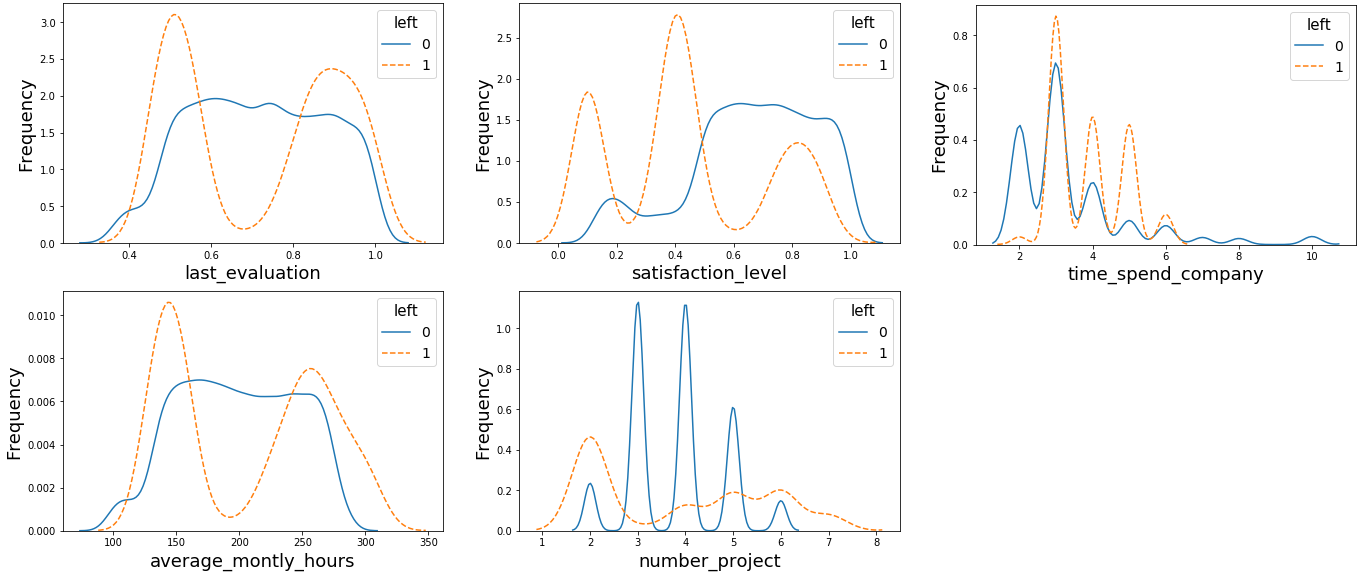
\includegraphics[width=0.9\textwidth]{distributions_by_left.png}
 \captionof{figure}{Distribuzione delle variabili numeriche rispetto al valore di left}
 \label{fig:distrib_by_left}
\end{center}

\noindent
La figura \ref{fig:time_by_sales} mostra invece come il tempo complessivo trascorso in azienda dagli impiegati che lavorano nel dipartimento \textit{'management'} è superiore alla media generale.

Infine, la figura \ref{fig:left_by_salary} testimonia un comportamento ragionevole degli impiegati: un reddito elevato è spesso una buona ragione per rimanere. Tra coloro che hanno un salario alto, infatti, sono pochi quelli che alla fine decidono di abbandonare il proprio posto di lavoro. Tra gli altri impiegati, invece, la percentuale di abbandono è decisamente più alta.


\noindent \begin{minipage}{\textwidth}

  \begin{minipage}[b]{0.50\textwidth}
    \centering

    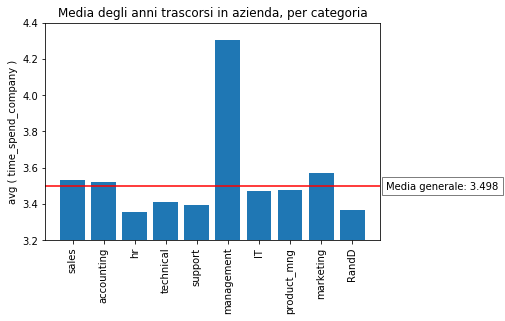
\includegraphics[width=\textwidth]{time_spent_by_sales}
    \captionof{figure}{Tempo medio trascorso in azienda, in base al dipartimento}
    \label{fig:time_by_sales}
  \end{minipage}
  \hfill
  \begin{minipage}[b]{0.45\textwidth}
    \centering

    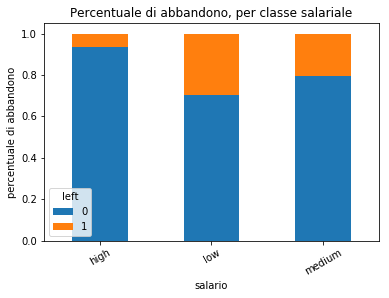
\includegraphics[width=\textwidth]{left_by_salary}
    \captionof{figure}{Percentuale di abbandono, per fascia di reddito}
        \label{fig:left_by_salary}
  \end{minipage}
  \end{minipage}


\subsection{Valutazione della qualità dei dati}

Come è possibile intuire dalla tabella \ref{tab:statistics}, nel dataset non ci sono valori mancanti. Inoltre, i singoli valori di ogni feature sono coerenti con i domini specificati nella tabella \ref{tab:semantics}: non sono dunque presenti errori dal punto di vista della sintassi dei dati (\textit{Syntactic Accuracy}).

Trattandosi di un dataset simulato, assumiamo anche l'accuratezza semantica dei dati (i dati rispecchiano una situazione reale e sono \textit{unbiased}), la completezza (coincidenza tra ciò che l'analisi richiede e ciò che i dati effettivamente raccontano) e la \textit{Timeliness} (nessun ritardo nella disponibilità dei dati).

 

\begin{center}
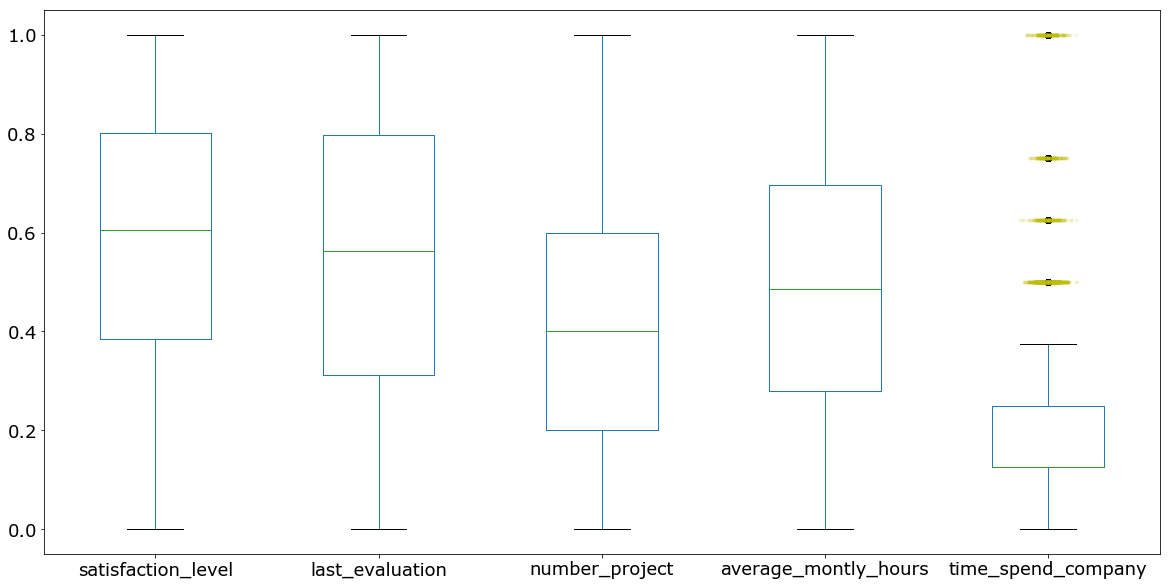
\includegraphics[width=0.8\textwidth]{box_plots.png}
\captionof{figure}{Rilevamento degli \textit{outliers}}
\label{fig:boxplots}
\end{center}

\noindent La figura \ref{fig:boxplots} illustra la distribuzione dei valori degli attributi numerici: notiamo che \texttt{number_project} assume per lo più valori minori o uguali alla metà del valore massimo (in questo caso 7, vedere la tabella \ref{tab:statistics}), mentre \texttt{time_spend_company} ha una distribuzione molto sbilanciata (il terzo quartile corrisponde al valore 4 e il valore massimo è 10, vedere ancora la tabella \ref{tab:statistics}). In più essa è anche l'unica feature per la quale sono presenti degli \textit{outlier}: nella figura \ref{fig:boxplots} è stato aggiunto del \textit{jitter} per avere un'idea della numerosità di tali valori. I suddetti \textit{outlier} corrispondono ai valori la cui frequenza nell'istogramma, rispetto alla frequenza degli altri valori, è bassa (figura \ref{fig:distrib_numer}, istogramma relativo a \texttt{time_spend_company}).

Avendo appurato l'assenza di problemi nella qualità dei dati (vedere le assunzioni fatte all'inizio di questo paragrafo) e vista la quantità non trascurabile di \textit{outlier}, è stato deciso di non escluderli dall'analisi.

\subsection{Trasformazione degli attributi}

A seconda delle necessità (formati di input richiesti da alcune librerie di supporto o semplicemente per rappresentare nella stessa scala diversi ordini di grandezza), talvolta i valori degli attributi numerici sono stati normalizzati nell'intervallo [0,1] e gli attributi categorici trasformati nei valori numerici corrispondenti. 

In altri contesti, invece, alcuni attributi sono stati scartati da una specifica parte dell'analisi (\texttt{promotion_last_5years} nella parte dell'\textit{Association Rules Mining}, per citarne uno) in quanto risultavano assai poco significativi.

Infine, nessuno degli attributi risulta essere legato ad altri da una stessa logica tale per cui sarebbe stato conveniente unirli in un unico attributo (per esempio tramite una funzione aritmetica che riassumesse più valori tramite una somma, differenza etc.), perciò nessuna trasformazione è stata effettuata in questa direzione. 

\subsection{Correlazione tra attributi ed eventuali variabili ridondanti}
L'indice di correlazione di \textit{Pearson} tra le coppie di attributi del dataset è rappresentato graficamente nella figura \ref{fig:corr_heatmap} (utilizzando una \textit{Heat Map}). Nella maggior parte dei casi, il livello di correlazione non supera la soglia del 30\% (si parla quindi di \textit{correlazione debole\footnote{https://it.wikipedia.org/wiki/Indice\_di\_correlazione\_di\_Pearson}}), mentre se ci si concentra sulle feature \texttt{last_evaluation}, \texttt{number_project} e \texttt{average_montly_hours} notiamo che il livello di correlazione tra di esse si alza di poco. Tuttavia, esso rimane ben al di sotto della soglia della \textit{correlazione forte} (che è del 70\%). 
Date le circostanze, dunque, è stata esclusa la presenza di variabili ridondanti: di conseguenza, nessuna feature è stata esclusa dall'analisi.
\begin{center}
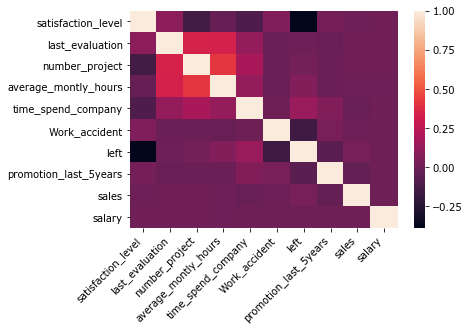
\includegraphics[width=0.7\textwidth]{corr_heatmap.png}
\captionof{figure}{Correlazione tra gli attributi (metrica di \textit{Pearson})}
\label{fig:corr_heatmap}
\end{center}

\section{Clustering}

\section{Pattern e Association Rules mining}

In questa sezione si presenta il processo di analisi delle \textit{Association Rules}. Inizialmente, si discutono alcune azioni preliminari effettuate sul dataset per preparare i dati alle operazioni successive. 
Dopodiché, si attua l'estrazione degli itemset frequenti (\textit{massimali}, \textit{chiusi} e \textit{frequenti}). 
Infine si estraggono da tali itemset le più interessanti regole di associazione, anche con lo scopo di costruire un modello di predizione per i valori mancanti e per l'attributo \texttt{left}.

\subsection{Operazioni preliminari}

Una delle operazioni propedeutiche alla fase di mining multidimensionale delle regole di associazione è la discretizzazione degli attributi numerici. Questa è stata effettuata in parte sulla base delle distribuzioni degli attributi in questione (quando ritenute interessanti) e in parte definendo intervalli di ampiezza fissata.

I valori dell'attributo \texttt{satisfaction\_level} sono stati raggruppati in quattro classi: \textit{very\_low}, per valori nell'intervallo [0, 0.25); \textit{low}, per valori nell'intervallo [0.25, 0.50); \textit{medium}, per valori nell'intervallo [0.50, 0.75); \textit{high}, per valori nell'intervallo [0.75, 1]. Tale suddivisione è stata ispirata dalla distribuzione lievemente irregolare dell'attributo (si veda la Figura \ref{fig:kdes}), che evidenzia un piccolo pinnacolo tra 0 e 0.25.

L'attributo \texttt{last\_evaluation} è stato invece discretizzato utilizzando intervalli di ampiezza 0.2, alla luce di una distribuzione priva di irregolarità ritenute significative.

Lo stesso vale per \texttt{average\_montly\_hours}, per il quale sono stati scelti intervalli di ampiezza 30. L'idea per la scelta di tale ampiezza è che un'ora (in media) di lavoro al giorno di differenza  sia una misura di discriminazione adeguata.

Dal momento che l'attributo \texttt{number\_project} presenta una distribuzione pressoché uniforme, si è scelto di discretizzarlo con intervalli di ampiezza fissata, in particolare 2, ritenendo che un solo progetto di differenza fosse una misura di discriminazione troppo "a grana fine", e che pertanto potesse dare origine a pattern frequenti e regole di associazione ridondanti.

Per la discretizzazione di \texttt{time\_spend\_company}, infine, la scelta dell'ampiezza degli intervalli riflette l'irregolarità della distribuzione (si veda la Figura \ref{fig:kdes}). Gli intervalli scelti, pensati appositamente per identificare tre categorie ben distinte di impiegati (che potremmo caratterizzare rispettivamente come quella degli impiegati recentemente assunti, quella di chi ha già alcuni anni alle spalle ed infine quella dei veterani), sono [2, 4), [4, 7) e [7, 10].

Per l'interpretazione dei valori discretizzati si faccia riferimento alla Tabella \ref{tab:legend}. I valori dell'attributo \path{sales} non hanno alcun suffisso in quanto identificabili senza alcuna ambiguità, mentre i valori per gli attributi \path{number_ project}, \path{average_montly_hours} e \path{last_evaluation} sono da intendersi come gli estremi sinistri del corrispondente intervallo di appartenenza (nel caso di \path{last_evaluation} il valore rappresenta una percentuale, perciò 50\_LE, ad esempio, indica in realtà un valore nell'intervallo [0.5, 0.7)). 

Prima di procedere con l'estrazione degli itemset frequenti e delle regole di associazione, si è deciso inoltre di rimuovere interamente l'attributo \path{promotion_last_5years}. La ragione di questa scelta è che oltre il 97\% delle righe del dataset hanno il medesimo valore dell'attributo, ossia 0. Ciò significa che la stragrande maggioranza degli itemset frequenti e delle regole di associazione registrerebbero il valore 0 per \path{promotion_last_5years}, il che appesantirebbe soltanto l'interpretazione degli itemset e delle regole senza rivelare alcuna proprietà interessante.

\begin{table}[h]
\centering
\begingroup
\setlength{\tabcolsep}{10pt} % Default value: 6pt
\renewcommand{\arraystretch}{1.5} % Default value: 1
\rowcolors{1}{grigio_chiaro}{white}
\begin{tabularx}{\textwidth}{|X|X|}
\hline
{\textbf{Suffisso}} & {\textbf{Attributo corrispondente}} \\
\_WA & Work\_accident \\
\_L & left \\
%\_PL5 & promotion\_last\_5years \\
\_SAT & satisfaction\_level \\
\_SAL & salary \\
\_LE & last\_evaluation \\
\_AMH & average\_montly\_hours \\
\_NP & number\_project \\
\_TSC & time\_spend\_company \\
\hline
\end{tabularx}
\endgroup
\caption{Legenda dei valori discretizzati}
\label{tab:legend}
\end{table}

\begin{figure}
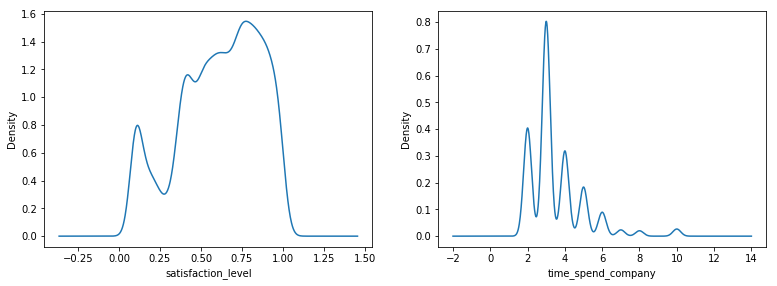
\includegraphics[width=\linewidth]{numerical_feat_distributions_new.png}

\caption{Kernel density estimation degli attributi satisfaction
\_level e time\_spend\_company.}
\label{fig:kdes}
\end{figure}


\subsection{Estrazione degli itemset frequenti}

Le sezioni che seguono sono dedicate all'estrazione delle diverse tipologie di itemset (massimali, chiusi e frequenti) con diversi valori del supporto. Nel caso degli itemset frequenti e chiusi si è scelto di restringere lo spazio di ricerca a quelli contenenti almeno tre elementi, mentre per quelli massimali il vincolo è di almeno due elementi. 
Per ogni intervallo di valori del supporto, i 10 itemset (quando disponibili) ritenuti più significativi sono stati riportati in una tabella. Di questi sono stati commentati i più interessanti.

\subsubsection{Itemset massimali}
Nella Tabella \ref{tab:maximal_15_20} sono riportati gli itemset massimali più significativi, estratti restringendo il valore del supporto tra 15 e 20 (in percentuale). Gli itemset 2 e 3 rivelano che una piccola percentuale degli impiegati che hanno trascorso pochi anni in azienda (da 2 a 3) - ed attualmente con un qualche incarico all'interno di essa - hanno un valore della valutazione tra 0.5 e 0.9. L'itemset 1 rivela, senza sorprese, che simili impiegati hanno concluso un numero di progetti relativamente basso (da 2 a 4). Il fatto che tutti gli itemset evidenzino l'assenza di incidenti sul lavoro è probabilmente imputabile alla distribuzione non omogenea dell'attributo \path{Work_accident}, che assume il valore 0 per più dell'80\% degli impiegati (si veda la Figura \ref{fig:distrib_categ} e la Tabella \ref{tab:statistics}).  

% MASSIMALI CON SUP DA 15 A 20
\begin{table}[h]
\centering
\begingroup
\setlength{\tabcolsep}{5pt} % Default value: 6pt
\renewcommand{\arraystretch}{1} % Default value: 1
\rowcolors{1}{grigio_chiaro}{white}
\setcounter{rowno}{0}
\begin{tabularx}{\textwidth}{|>{\stepcounter{rowno}\therowno}c|X|c|}
\hline
\multicolumn{1}{|r}{\#} & {\textbf{Itemset}} & {\textbf{Supporto (\%)}} \\

& \{2\_NP, 2\_to\_3\_TSC, 0\_L, 0\_WA\} & 19.5946 \\ 
& \{50\_LE, 2\_to\_3\_TSC, 0\_L, 0\_WA\} & 17.7945 \\ 
& \{70\_LE, 2\_to\_3\_TSC, 0\_L, 0\_WA\} & 15.5677 \\ 
& \{4\_to\_6\_TSC, 0\_L, 0\_WA\} & 15.4277 \\ 

\hline
\end{tabularx}
\endgroup
\caption{Itemset massimali con supporto tra 15\% e 20\%}
\label{tab:maximal_15_20}
\end{table}

\noindent
Nella Tabella \ref{tab:maximal_10_15} sono invece registrati gli itemset massimali con supporto tra 10 e 15.
Tra i più interessanti troviamo i numeri 5 e 6, che rispettivamente registrano, per alcuni degli impiegati con un salario basso, l'abbandono dell'impiego (come è lecito aspettarsi) ed un valore alto dell'ultima valutazione (rivelando un dato insapettato), e il numero 7, il quale suggerisce che, per una percentuale non trascurabile di impiegati, un incidente sul lavoro non influisce sulla di questi volontà di mantenere il posto in azienda. 
La considerazione fatta in precendenza circa l'assidua presenza di 0\_WA negli itemset trova in questo caso un ulteriore riscontro.

% MASSIMALI CON SUP DA 10 A 15
\begin{table}[h]
\centering
\begingroup
\setlength{\tabcolsep}{5pt} % Default value: 6pt
\renewcommand{\arraystretch}{1} % Default value: 1
\rowcolors{1}{grigio_chiaro}{white}
\setcounter{rowno}{0}

\begin{tabularx}{\textwidth}{|>{\stepcounter{rowno}\therowno}c|X|c|}
\hline
\multicolumn{1}{r}{\#} & {\textbf{Itemset}} & {\textbf{Supporto (\%)}} \\
 
& \{2\_NP, low\_SAL, 2\_to\_3\_TSC, 0\_WA\} & 14.8077 \\ 
& \{4\_to\_6\_TSC, 4\_NP, 0\_WA\} & 14.541 \\ 
& \{4\_to\_6\_TSC, low\_SAL, 0\_WA\} & 14.2543 \\ 
& \{50\_LE, 2\_NP, 2\_to\_3\_TSC, 0\_WA\} & 14.1476 \\ 
& \{1\_L, low\_SAL, 0\_WA\} & 13.8476 \\ 
& \{70\_LE, low\_SAL, 0\_WA\} & 13.6876 \\ 
& \{1\_WA, 0\_L\} & 13.3342 \\ 
& \{150\_AMH, 0\_L, 0\_WA\} & 13.2942 \\ 
& \{150\_AMH, 2\_to\_3\_TSC, 0\_WA\} & 13.0475 \\ 
& \{50\_LE, 4\_NP, 0\_L, 0\_WA\} & 12.6808 \\ 
 
\hline
\end{tabularx}
\endgroup
\caption{Itemset massimali con supporto tra 10\% e 15\%}
\label{tab:maximal_10_15}
\end{table}

\noindent
Itemset massimali con supporto maggiore o uguale a 20 non sono stati rilevati.



\subsubsection{Itemset chiusi}

Gli unici due itemset chiusi con supporto superiore al 30\% sono contenuti nella Tabella \ref{tab:closed_sup_30_101}. Il numero 1 rivela che una buona frazione degli impiegati (circa il 44 \%) è costituita da coloro che hanno trascorso poco tempo in azienda, non sono stati vittime di incidenti e mantengono tuttora il loro incarico. Essi potrebbero rappresentare i tipici nuovi arrivati. Il numero 2 cattura un altrettanto buona porzione di impiegati aventi caratteristiche simili (nessun incidente e nessun abbandono del lavoro) ed un numero di progetti portati a termine tra 4 e 5.

% CHIUSI CON SUP OLTRE 30
\begin{table}[h]
\centering
\begingroup
\setlength{\tabcolsep}{5pt} % Default value: 6pt
\renewcommand{\arraystretch}{1} % Default value: 1
\rowcolors{1}{grigio_chiaro}{white}
\setcounter{rowno}{0}

\begin{tabularx}{\textwidth}{|>{\stepcounter{rowno}\therowno}c|X|c|}
\hline
\multicolumn{1}{r}{\#} & {\textbf{Itemset}} & {\textbf{Supporto (\%)}} \\

& \{2\_to\_3\_TSC, 0\_L, 0\_WA\} & 44.4696 \\
& \{4\_NP, 0\_L, 0\_WA\} & 33.7489 \\ 
 
\hline
\end{tabularx}
\endgroup
\caption{Itemset chiusi con supporto maggiore del 30\%}
\label{tab:closed_sup_30_101}
\end{table}

Gli itemset chiusi con supporto tra 20\% e 30\% possono essere osservati nella Tabella \ref{tab:closed_sup_20_30}. Similmente ad alcuni itemset riportati e discussi precedentemente, il numero 1 rivela caratteristiche non troppo sorprendenti di quelli che sembrano essere gli impiegati con un trascorso breve all'interno dell'azienda: un basso numero di progetti realizzati (2 o 3), pochi anni di esperienza (2 o 3) e nessun incidente lavorativo. Il numeri 3 e 6 sembrano invece identificare due prototipi dell'impiegato standard, da una parte accomunati dall'assenza di incidenti e dalla permanenza in azienda, dall'altra contraddistinti rispettivamente da un salario medio e da un livello medio di soddisfazione. I numeri 4 e 5 rappresentano due categorie simili di impiegati, concordanti sul salario basso e sull'assenza di incidenti lavorativi, ma con le rispettive peculiarità di non aver abbandonato il lavoro (nonostante il salario basso) e di aver passato da 2 a 3 anni in azienda (che potrebbe suggerire che salari medi ed alti siano riservati a chi ha più esperienza).


% CHIUSI CON SUP TRA 20 E 30
\begin{table}[h]
\centering
\begingroup
\setlength{\tabcolsep}{5pt} % Default value: 6pt
\renewcommand{\arraystretch}{1} % Default value: 1
\rowcolors{1}{grigio_chiaro}{white}
\setcounter{rowno}{0}

\begin{tabularx}{\textwidth}{|>{\stepcounter{rowno}\therowno}c|X|c|}
\hline
\multicolumn{1}{r}{\#} & {\textbf{Itemset}} & {\textbf{Supporto (\%)}} \\

& \{2\_NP, 2\_to\_3\_TSC, 0\_WA\} & 29.4753 \\ 
& \{4\_NP, 2\_to\_3\_TSC, 0\_L\} & 28.6886 \\ 
& \{medium\_SAL, 0\_L, 0\_WA\} & 28.4419 \\ 
& \{low\_SAL, 0\_L, 0\_WA\} & 27.9952 \\ 
& \{low\_SAL, 2\_to\_3\_TSC, 0\_WA\} & 26.8418 \\ 
& \{medium\_SAT, 0\_L, 0\_WA\} & 26.4284 \\ 
& \{2\_NP, 0\_L, 0\_WA\} & 26.3084 \\ 
& \{low\_SAL, 2\_to\_3\_TSC, 0\_L\} & 24.8283 \\ 
& \{high\_SAT, 0\_L, 0\_WA\} & 24.6616 \\ 
& \{medium\_SAT, 2\_to\_3\_TSC, 0\_L\} & 24.2683 \\ 

\hline
\end{tabularx}
\endgroup
\caption{Itemset chiusi con supporto tra 20\% e 30\%}
\label{tab:closed_sup_20_30}
\end{table}



\subsubsection{Itemset frequenti}

La Tabella \ref{tab:frequent_sup_20_101} mostra gli itemset frequenti con supporto superiore al 20\%. Il fatto che nessuno di questi abbia un supporto maggiore o uguale al 25\% può sembrare contraddittorio, visto che gli itemset frequenti sono un sovrainsieme degli itemset massimali e chiusi elencati in precedenza. In realtà, ciò è dovuto al fatto che sono pochi gli itemset propriamente frequenti, ossia non chiusi. Per questo, gli itemset frequenti con supporto maggiore del 25\% che sembrano "mancanti" sono in realtà chiusi e, in quanto tali, non sono stati riportati una seconda volta sotto la sezione degli itemset frequenti.

Cercando di individuare gli itemset più significativi, il numero 1 testimonia che una buona percentuale di impiegati caratterizzati da una breve permanenza in azienda (2 o 3 anni) sono riusciti a portare a termine un discreto numero di progetti (4 o 5) senza incorrere in incidenti. Ciò fa pensare a progetti relativamente semplici ed esenti da rischi. Il numero 6 rivela invece l'esistenza di alcuni impiegati che, malgrado i pochi anni trascorsi nella compagnia, sono riusciti ad ottenere un salario medio e compatibilmente scelgono di mantenere il posto di lavoro. Una categoria analoga di persone è identificata dall'itemset numero 8, con l'unica differenza che, al posto di un salario medio, questa include coloro che possono ritenersi soddisfatti del loro impiego (alto livello di soddisfazione). 

% FREQUENTI CON SUP OLTRE 20
\begin{table}[h]
\centering
\begingroup
\setlength{\tabcolsep}{5pt} % Default value: 6pt
\renewcommand{\arraystretch}{1} % Default value: 1
\rowcolors{1}{grigio_chiaro}{white}
\setcounter{rowno}{0}

\begin{tabularx}{\textwidth}{|>{\stepcounter{rowno}\therowno}c|X|c|}
\hline
\multicolumn{1}{r}{\#} & {\textbf{Itemset}} & {\textbf{Supporto (\%)}} \\

& \{4\_NP, 2\_to\_3\_TSC, 0\_WA\} & 24.2283 \\ 
& \{50\_LE, 2\_to\_3\_TSC, 0\_WA\} & 24.1216 \\ 
& \{50\_LE, 0\_L, 0\_WA\} & 23.9416 \\ 
& \{4\_NP, 2\_to\_3\_TSC, 0\_L, 0\_WA\} & 23.8416 \\ 
& \{2\_NP, 2\_to\_3\_TSC, 0\_L\} & 23.7349 \\ 
& \{medium\_SAL, 2\_to\_3\_TSC, 0\_L\} & 23.6482 \\ 
& \{medium\_SAL, 2\_to\_3\_TSC, 0\_WA\} & 23.4816 \\ 
& \{high\_SAT, 2\_to\_3\_TSC, 0\_L\} & 22.6215 \\ 
& \{70\_LE, 0\_L, 0\_WA\} & 22.3882 \\ 
& \{50\_LE, 2\_to\_3\_TSC, 0\_L\} & 21.3014 \\ 

\hline
\end{tabularx}
\endgroup
\caption{Itemset frequenti con supporto maggiore del 20\%}
\label{tab:frequent_sup_20_101}
\end{table}


La Tabella \ref{tab:frequent_sup_10_20} registra invece gli itemset frequenti con valore del supporto tra 10\% e 20\%. Il numero 4 mette in luce un gruppo di impiegati che sono riusciti a soddisfare le aspettative dell'azienda, totalizzando un punteggio tra 0.7 e 0.9 nell'ultima valutazione, nonostante un trascorso breve. Senza sorprese, tali impiegati scelgono di non lasciare il lavoro. Questa categoria di dipendenti potrebbe rappresentare coloro che sono partiti "col piede giusto". Il numero 6 cattura invece un insieme di persone aventi un alto livello di soddisfazione ed numero di progetti completati compreso tra 4 e 5, il tutto accompagnato dall'assenza di incidenti sul posto di lavoro. Per questi impiegati è possibile concludere che soddisfazione e produttività vanno di pari passo.  

% FREQUENTI CON SUP TRA 10 E 20
\begin{table}[h]
\centering
\begingroup
\setlength{\tabcolsep}{5pt} % Default value: 6pt
\renewcommand{\arraystretch}{1} % Default value: 1
\rowcolors{1}{grigio_chiaro}{white}
\setcounter{rowno}{0}

\begin{tabularx}{\textwidth}{|>{\stepcounter{rowno}\therowno}c|X|c|}
\hline
\multicolumn{1}{r}{\#} & {\textbf{Itemset}} & {\textbf{Supporto (\%)}} \\

& \{medium\_SAL, 2\_to\_3\_TSC, 0\_L, 0\_WA\} & 19.7813 \\ 
& \{4\_NP, low\_SAL, 0\_WA\} & 19.1813 \\ 
& \{high\_SAT, 2\_to\_3\_TSC, 0\_WA\} & 18.9879 \\ 
& \{70\_LE, 2\_to\_3\_TSC, 0\_L\} & 18.9613 \\ 
& \{high\_SAT, 2\_to\_3\_TSC, 0\_L, 0\_WA\} & 18.8346 \\ 
& \{high\_SAT, 4\_NP, 0\_WA\} & 18.8013 \\ 
& \{4\_NP, low\_SAL, 0\_L\} & 18.5612 \\ 
& \{medium\_SAL, 4\_NP, 0\_L\} & 18.1679 \\ 
& \{2\_NP, low\_SAL, 0\_WA\} & 17.9812 \\ 
& \{medium\_SAL, 4\_NP, 0\_WA\} & 17.5612 \\ 
\hline
\end{tabularx}
\endgroup
\caption{Itemset frequenti con supporto tra 10\% e 20\%}
\label{tab:frequent_sup_10_20}
\end{table}



\subsection{Estrazione delle regole di associazione}

Di seguito si riportano le regole di associazione estratte per differenti valori della confidenza. Al fine di limitare il numero di regole restituite, si è scelto di generarle a partire da itemset frequenti di lunghezza maggiore o uguale a 3. 
Per ogni intervallo di valori della confidenza, le 10 regole ritenute più significative sono state riportate in una tabella, quindi si è proceduto a commentare quelle più interessanti. In ciascuna tabella è possibile distinguere tre categorie di regole:
\begin{itemize}
\setlength\itemsep{1pt}
\item regole "generiche", la cui conseguenza rivela un dato riguardante un attributo diverso da \path{left}
\item regole la cui conseguenza rivela l'abbandono del posto di lavoro (\path{left}=1)
\item regole la cui conseguenza rivela il mantenimento del posto di lavoro (\path{left}=0)
\end{itemize}
\noindent
La Tabella \ref{tab:rules_conf_90_101} riporta le regole con confidenza maggiore del 90\%. La numero 3 indica che poche ore di lavoro (da 120 a 150 al mese), combinate con un piccolo numero di progetti completati (2 o 3), una breve permanenza in azienda e l'abbandono dell'impiego, determinano quasi certamente (con una confidenza maggiore del 99\%) un basso livello di soddisfazione. La numero 4 varia la causa sostituendo le poche ore di lavoro con un valore dell'ultima valutazione tra 0.5 e 0.7, rivelando la medesima conseguenza. 
La numero 8 evidenzia una delle principali combinazioni di fattori che portano all'abbandono del posto di lavoro, ossia un gran numero di progetti completati, una permanenza in azienda compresa tra 4 e 6 anni, nonché un livello di soddisfazione molto basso. A questi va aggiunto anche il non verificarsi di incidenti, come a sottolineare che non si tratta del vero motivo per cui gli impiegati decidono di andarsene. Questa regola suggerisce che nel lungo termine i dipendenti sono più propensi a lasciare il lavoro. La numero 9, invece, indica che un alto livello di soddisfazione tra quelli che potremmo definire i neo assunti (ossia che hanno trascorso dai 2 ai 3 anni in azienda) fa sì che questi scelgano di rimanere.

%REGOLE CON CONF TRA 90 E 100
\begin{table}[h]
\centering
\begingroup
\setlength{\tabcolsep}{5pt} % Default value: 6pt
\renewcommand{\arraystretch}{1} % Default value: 1
\rowcolors{1}{grigio_chiaro}{white}
\setcounter{rowno}{0}

\begin{tabularx}{\textwidth}{|>{\stepcounter{rowno}\therowno}c|X|l|c|c|}
\hline
\multicolumn{1}{r}{\#} & {\textbf{Premessa}} & {\textbf{Conseguenza}} & {\textbf{Lift (\%)}} & {\textbf{Confidenza (\%)}} \\

& \{very\_low\_SAT, 1\_L, 4\_to\_6\_TSC\} & 6\_NP & 982.029 & 93.6264 \\ 
& \{6\_NP, 1\_L, 4\_to\_6\_TSC\} & very\_low\_SAT & 829.409 & 96.1625 \\ 
& \{120\_AMH, 1\_L, 2\_NP, 2\_to\_3\_TSC\} & low\_SAT & 526.352 & 99.803 \\ 
& \{1\_L, 50\_LE, 2\_NP, 2\_to\_3\_TSC\} & low\_SAT & 522.447 & 99.0625 \\ 
& \{6\_NP, very\_low\_SAT, 1\_L\} & 4\_to\_6\_TSC & 312.963 & 99.0698 \\ 
& \{120\_AMH, low\_SAT, 1\_L, 2\_to\_3\_TSC\} & 2\_NP & 231.198 & 99.3137 \\ 
& \{120\_AMH, low\_SAT, 2\_NP, 2\_to\_3\_TSC\} & 1\_L & 383.663 & 91.3436 \\ 
& \{6\_NP, very\_low\_SAT, 4\_to\_6\_TSC, 0\_WA\} & 1\_L & 379.931 & 90.455 \\ 
& \{high\_SAT, 2\_to\_3\_TSC\} & 0\_L & 130.326 & 99.2976 \\ 
& \{4\_NP, 2\_to\_3\_TSC\} & 0\_L & 129.473 & 98.6474 \\ 
\hline
\end{tabularx}
\endgroup
\caption{Regole di associazione con confidenza maggiore del 90\%}
\label{tab:rules_conf_90_101}
\end{table}

La Tabella \ref{tab:rules_conf_80_90} riporta le regole con confidenza tra l'80\% e il 90\%. La regola 1 mette in risalto un dato molto interessante: un numero di progetti tra 6 e 7, accompagnato da una permanenza relativamente lunga (da 4 a 6 anni), comporta un livello di soddisfazione molto basso. Ciò rivela un'informazione preziosa per l'azienda: i dipendenti con più esperienza non si ritengono affatto soddisfatti della loro attuale situazione, pertanto è bene correre ai ripari. La numero  4 suggerisce che le cause di una scarsa efficienza (solo 2 o 3 progetti completati) sono un livello di soddisfazione basso ed un punteggio medio basso (da 0.3 a 0.5) nell'ultima valutazione. È probabile quindi che una migliore produttività si possa ottenere a fronte di incentivi da parte della compagnia, siano essi diretti (fornire un punteggio maggiore nella valutazione) o indiretti (cercare di aumentare il livello di soddisfazione dei lavoratori). La regola 7 mostra che un numero di ore mensili compreso tra 120 e 150, un numero di progetti realizzati compreso tra 2 e 3 ed un basso livello di soddisfazione causano nell'88\% dei casi l'abbandono del posto di lavoro. Contrariamente, la regola 10 afferma che un livello di soddisfazione alto ed un contesto lavorativo sicuro sono fattori che determinano il mantenimento del posto di lavoro. 

%REGOLE CON CONF TRA 80 E 90
\begin{table}[h]
\centering
\begingroup
\setlength{\tabcolsep}{4pt} % Default value: 6pt
\renewcommand{\arraystretch}{1} % Default value: 1
\rowcolors{1}{grigio_chiaro}{white}
\setcounter{rowno}{0}

\begin{tabularx}{\textwidth}{|>{\stepcounter{rowno}\therowno}c|X|l|c|c|}
\hline
\multicolumn{1}{r}{\#} & {\textbf{Premessa}} & {\textbf{Conseguenza}} & {\textbf{Lift (\%)}} & {\textbf{Confidenza (\%)}} \\

& \{6\_NP, 4\_to\_6\_TSC\} & very\_low\_SAT & 704.962 & 81.734 \\ 
& \{120\_AMH, 2\_NP, low\_SAL, 2\_to\_3\_TSC, 0\_WA\} & low\_SAT & 425.47 & 80.6744 \\ 
& \{low\_SAT, 50\_LE, low\_SAL\} & 2\_NP & 201.126 & 86.3962 \\ 
& \{30\_LE, low\_SAT\} & 2\_NP & 197.358 & 84.7775 \\ 
& \{sales, 2\_NP, low\_SAL\} & 2\_to\_3\_TSC & 126.594 & 81.7597 \\ 
& \{4\_to\_6\_TSC, high\_SAT, 4\_NP\} & 0\_WA & 105.14 & 89.9356 \\ 
& \{120\_AMH, low\_SAT, 2\_NP\} & 1\_L & 371.404 & 88.4247 \\ 
& \{6\_NP, very\_low\_SAT, 4\_to\_6\_TSC\} & 1\_L & 368.547 & 87.7446 \\ 
& \{medium\_SAL, 4\_NP\} & 0\_L & 115.037 & 87.6488 \\ 
& \{high\_SAT, 0\_WA\} & 0\_L & 108.829 & 82.9186 \\ 
\hline
\end{tabularx}
\endgroup
\caption{Regole di associazione con confidenza tra 80\% e 90\%}
\label{tab:rules_conf_80_90}
\end{table}

Nella Tabella \ref{tab:rules_conf_70_80} sono elencate le regole con confidenza compresa tra 70\% ed 80\%. La regola 5 rivela che gli impiegati con un trascorso piuttosto lungo (da 4 a 6 anni), un numero di progetti alle spalle compreso tra 4 e 5, un punteggio molto alto nell'ultima valutazione (tra 0.9 e 1) e nessun incidente si ritengono, nella maggior parte dei casi (circa 70\%), molto soddisfatti. Questo suggerisce che i dipendenti prediligono un carico di lavoro relativamente basso (circa 1 progetto all'anno), il quale consente loro, peraltro, di ottenere un'ottima valutazione da parte dell'azienda. La regola 7 mette invece in evidenza il fatto che un salario ed un livello di soddisfazione bassi, abbinati ad una produttività mediocre (2 o 3 progetti completati), determina la perdita dell'impiego. La regola 10, infine, dimostra che gli impiegati assunti da poco tempo sono tendenzialmente disposti ad accettare un salario basso pur di mantenere il loro posto in azienda.

%REGOLE CON CONF TRA 70 E 80
\begin{table}[h]
\centering
\begingroup
\setlength{\tabcolsep}{5pt} % Default value: 6pt
\renewcommand{\arraystretch}{1} % Default value: 1
\rowcolors{1}{grigio_chiaro}{white}
\setcounter{rowno}{0}

\begin{tabularx}{\textwidth}{|>{\stepcounter{rowno}\therowno}c|X|l|c|c|}
\hline
\multicolumn{1}{r}{\#} & {\textbf{Premessa}} & {\textbf{Conseguenza}} & {\textbf{Lift (\%)}} & {\textbf{Confidenza (\%)}} \\

& \{very\_low\_SAT, 4\_to\_6\_TSC, 70\_LE\} & 6\_NP & 764.086 & 72.8477 \\ 
& \{6\_NP, low\_SAL\} & very\_low\_SAT & 663.809 & 76.9627 \\ 
& \{30\_LE, 2\_NP, 2\_to\_3\_TSC\} & low\_SAT & 409.318 & 77.6119 \\ 
& \{1\_L, 4\_to\_6\_TSC, 4\_NP\} & high\_SAT & 223.705 & 78.7942 \\ 
& \{90\_LE, 4\_to\_6\_TSC, 4\_NP, 0\_WA\} & high\_SAT & 199.63 & 70.3145 \\ 
& \{low\_SAT, low\_SAL\} & 2\_NP & 185.483 & 79.6764 \\ 
& \{low\_SAT, 2\_NP, low\_SAL\} & 1\_L & 324.144 & 77.173 \\ 
& \{6\_NP, 4\_to\_6\_TSC\} & 1\_L & 313.249 & 74.5791 \\ 
& \{70\_LE, 0\_WA\} & 0\_L & 103.409 & 78.7893 \\ 
& \{low\_SAL, 2\_to\_3\_TSC\} & 0\_L & 103.29 & 78.6982 \\ 
\hline
\end{tabularx}
\endgroup
\caption{Regole di associazione con confidenza tra 70\% e 80\%}
\label{tab:rules_conf_70_80}
\end{table}

\subsubsection{Predizione dei valori mancanti}

In assenza di valori mancanti all'interno del dataset, si è scelto di introdurne appositamente alcuni. In particolare, si è tentato di predire, utilizzando le regole più significative, i valori dell'attributo \path{Work_accident} per una frazione del dataset originale. A questo scopo, si è adottato il seguente procedimento: per prima cosa è stato estratto in maniera casuale il 10\% delle righe (mantenendo la distribuzione relativa dei valori dell'attributo \path{Work_accident}). Fatto ciò, sono state estratte le regole di associazione aventi rispettivamente \path{0_WA} e \path{1_WA} nella conseguenza, restringendo il campo a quelle con valore della confidenza maggiore o uguale al 70\%. Per ottenere l'insieme di regole riportate nella Tabella \ref{tab:rules_predict_missing} sono state estratte le prime 5 regole (ordinate secondo il valore del lift) di ciascuno dei due insiemi. Si noti che nella tabella non appare nessuna regola avente \path{1_WA} come valore della conseguenza, questo perché nessuna regola con tali caratteristiche è stata restituita da Apriori. La predizione dei valori mancanti con tale insieme di regole raggiunge un'accuratezza del 98.4\%. Qualora si desiderasse ripetere l'esperimento, è sufficiente estrarre casualmente il 10\% delle righe del dataset (avendo l'accortezza di preservare la distribuzione relativa dei valori di \path{Work_accident}) utilizzando la funzione Python  \path{pandas.DataFrame.sample} e impostando il valore del parametro \path{random_state} a 1.

\begin{table}[h]
\centering
\begingroup
\setlength{\tabcolsep}{5pt} % Default value: 6pt
\renewcommand{\arraystretch}{1} % Default value: 1
\rowcolors{1}{grigio_chiaro}{white}
\setcounter{rowno}{0}

\begin{tabularx}{\textwidth}{|>{\stepcounter{rowno}\therowno}c|X|l|c|c|}
\hline
\multicolumn{1}{r}{\#} & {\textbf{Premessa}} & {\textbf{Conseguenza}} & {\textbf{Lift (\%)}} & {\textbf{Confidenza (\%)}} \\

& \{120\_AMH, low\_SAT, 1\_L\} & 0\_WA & 112.284 & 96.0463 \\ 
& \{90\_LE, 1\_L, 4\_to\_6\_TSC\} & 0\_WA & 112.265 & 96.03 \\ 
& \{90\_LE, 1\_L\} & 0\_WA & 112.259 & 96.0251 \\ 
& \{120\_AMH, low\_SAT, 1\_L, 2\_to\_3\_TSC\} & 0\_WA & 112.207 & 95.9804 \\ 
& \{120\_AMH, low\_SAT, 1\_L, 2\_NP\} & 0\_WA & 112.188 & 95.9646 \\ 

\hline
\end{tabularx}
\endgroup
\caption{Regole di associazione usate per predire il valore di Work\_accident}
\label{tab:rules_predict_missing}
\end{table}

\subsubsection{Predizione dell'attributo 'left'}

Per predire i valori dell'attributo \path{left} si è proceduto in maniera del tutto analoga. Regole aventi il valore \path{1_L} e \path{0_L} nella conseguenza sono state separatamente estratte ed ordinate secondo il valore del lift. Da ciascuno dei due insiemi ordinati sono state estratte le prime 5 regole, le quali sono state combinate per ottenere l'insieme mostrato nella Tabella \ref{tab:rules_predict_left}. L'impiego di tali regole per la predizione dei valori di \path{left} (attenendosi al verdetto della maggioranza nel caso di più regole compatibili con una stessa riga del dataset) permette di raggiungere un'accuratezza del 96.7\%.

\begin{table}[h]
\centering
\begingroup
\setlength{\tabcolsep}{5pt} % Default value: 6pt
\renewcommand{\arraystretch}{1} % Default value: 1
\rowcolors{1}{grigio_chiaro}{white}
\setcounter{rowno}{0}

\begin{tabularx}{\textwidth}{|>{\stepcounter{rowno}\therowno}c|X|l|c|c|}
\hline
\multicolumn{1}{r}{\#} & {\textbf{Premessa}} & {\textbf{Conseguenza}} & {\textbf{Lift (\%)}} & {\textbf{Confidenza (\%)}} \\

& \{120\_AMH, low\_SAT, 2\_NP, 2\_to\_3\_TSC, 0\_WA\} & 1\_L & 388.451 & 92.4833 \\ 
& \{120\_AMH, low\_SAT, 2\_NP, 2\_to\_3\_TSC\} & 1\_L & 383.663 & 91.3436 \\ 
& \{6\_NP, very\_low\_SAT, 4\_to\_6\_TSC, 0\_WA\} & 1\_L & 379.931 & 90.455 \\ 
& \{120\_AMH, low\_SAT, 2\_NP, 0\_WA\} & 1\_L & 377.439 & 89.8618 \\ 
& \{120\_AMH, low\_SAT, 2\_to\_3\_TSC, 0\_WA\} & 1\_L & 375.184 & 89.3248 \\ 
& \{high\_SAT, 2\_to\_3\_TSC\} & 0\_L & 130.326 & 99.2976 \\ 
& \{medium\_SAT, 2\_to\_3\_TSC\} & 0\_L & 129.786 & 98.8862 \\ 
& \{medium\_SAT, 2\_to\_3\_TSC, 0\_WA\} & 0\_L & 129.521 & 98.6842 \\ 
& \{4\_NP, 2\_to\_3\_TSC\} & 0\_L & 129.473 & 98.6474 \\ 
& \{4\_NP, 2\_to\_3\_TSC, 0\_WA\} & 0\_L & 129.153 & 98.404 \\ 

\hline
\end{tabularx}
\endgroup
\caption{Regole di associazione usate per predire il valore di left}
\label{tab:rules_predict_left}
\end{table}



\section{Classificazione}

In questa sezione si illustra il processo di classificazione. L'obiettivo è quello di costruire un modello basato su \textit{Decision tree} e utilizzarlo per prevedere se, a partire dai valori di alcuni suoi attributi, un impiegato dell'azienda lascerà o meno il lavoro. Nello specifico, gli attributi utilizzati in questa sede sono \texttt{satisfaction_level, last_evaluation, number_project, average_montly_hours, time_spend_company, Work_accident, salary}. Tra questi attributi, quelli categorici sono stati codificati con valori interi. 
\'E stato deciso di non prendere in considerazione l'attributo categorico non ordinale \texttt{sales} perché il suo valore risultava, nella maggior parte dei casi, totalmente ininfluente nel processo di decisione. L'importanza di tale feature nei processi di decisione dei modelli 1, 2, 3, 4 (illustrati nel seguito), infatti, è di 0, 0, 0 e 0.005 rispettivamente. 

\subsection{Classificazione tramite alberi di decisione}

Nel seguito sono riportate le performance di diversi alberi di decisione, ognuno dei quali presenta una diversa configurazione dei parametri di learning. I parametri utilizzato sono i seguenti:

\begin{itemize}
\setlength\itemsep{0.30em}
	\item \texttt{criterion:} Criterio con cui misurare la qualità di una suddivisione. I valori possibili sono \texttt{gini} (Gini impurity) e \texttt{entropy} (per l'information gain)
	
	\item \texttt{max_depth:} La massima profondità dell'albero. Se inizializzato a \texttt{None}, le suddivisioni sono attuate finché tutte le foglie non sono pure o contengono un numero di record minore di \texttt{min_samples_split}
	
	\item \texttt{min_samples_split:} Numero minimo di record necessario per suddividere un nodo intermedio
	
	\item \texttt{min_samples_leaf:} Numero minimo di record che le foglie devono contenere
	
	\item \texttt{class_weight:} Peso assegnato alle classi, utilizzato al momento della scelta della suddivisione migliore. Se il valore specificato è \texttt{None}, il peso di tutte le classi è considerato uguale a 1.
\end{itemize}

\noindent Nelle rappresentazioni grafiche dei modelli, un colore scuro di un nodo dell'albero corrisponde a un valore basso di \texttt{gini}/\texttt{entropy}. Al contrario, un colore chiaro indica un valore alto.

\subsubsection*{Modello 1}

L'unico vincolo di questo modello riguarda la massima profondità dell'albero.
Il modello nella figura \ref{img:model1} opera una prima suddivisione dei record in base al valore dell'attributo \texttt{satisfaction_level}: quelli aventi un valore maggiore di 0.465 sono classificati come \texttt{Not left} (questa scelta risulta abbastanza intuitiva). Se invece \texttt{satisfaction_level} assume un valore minore o uguale a 0.465, allora il modello controlla anche il valore dell'attributo \texttt{number_project}: se un impiegato ha portato a termine più di 2 progetti, allora viene classificato come \texttt{Not left}. In caso contrario, viene attribuito alla classe \texttt{Left}.\newline\bigskip

\noindent\begin{minipage}{\textwidth}

  \begin{minipage}[b]{0.65\textwidth}
    \centering
    \label{img:model1}
    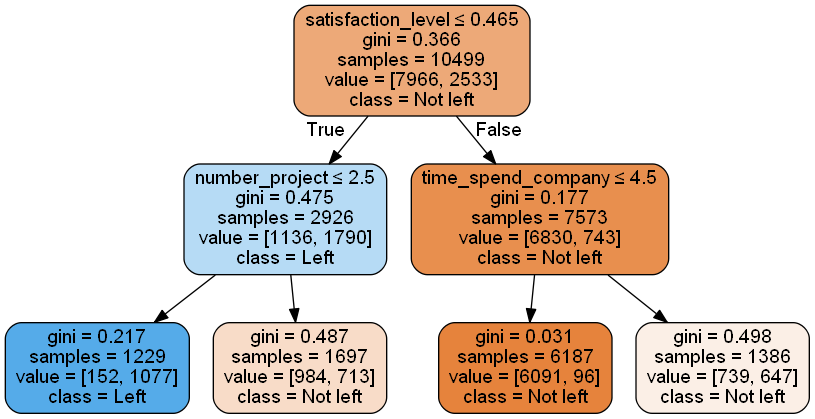
\includegraphics[width=\textwidth]{albero4}
    \captionof{figure}{Rappresentazione grafica del modello}
  \end{minipage}
  \hfill
  \begin{minipage}[b]{0.3\textwidth}
    \centering
    \setlength{\tabcolsep}{10pt} % Default value: 6pt
\renewcommand{\arraystretch}{1.5} % Default value: 1
\rowcolors{1}{grigio_chiaro}{white}
    \begin{tabularx}{\textwidth}{|lX|}
	\hline
	criterion                & gini      \\
	max\_depth               & 2         \\
	min\_samples\_split      & 2         \\
	min\_samples\_leaf       & 2         \\
	class\_weight            & None     \\\hline
	\end{tabularx}
      \captionof{table}{Parametri del modello}
    \end{minipage}
  \end{minipage}

\subsubsection*{Modello 2}

Per questo modello è stato deciso di rilassare leggermente il vincolo sulla profondità massima ed è stato deciso di assegnare un peso diverso a ciascuna delle due classi (in accordo alla distribuzione dei valori della feature \texttt{left}).
Il modello nella figura \ref{img:model2}, come il precedente, effettua inizialmente una suddivisione basandosi sull'attributo \texttt{satisfaction_level}: 
\begin{itemize}
\item se l'impiegato ha un livello di soddisfazione inferiore o uguale a 0.465, il modello controlla \texttt{time_spend_company}. Per un valore minore o uguale a 4.5, il modello tende ad assegnare l'etichetta \texttt{Left} (la successiva divisione si basa di nuovo su \texttt{time_spend_company}). Altrimenti assegna nella maggior parte dei casi l'etichetta \texttt{Not left} (con la successiva suddivisione su \texttt{satisfaction_level}
\item se invece il livello di soddisfazione è superiore a 0.465, il modello controlla di nuovo \texttt{time_spend_company}: al contrario di prima, per un valore minore o uguale a 4.5, il modello assegna alla maggior parte dei record la classe \texttt{Not left} (divisione successiva: \texttt{number_projects}). Per un valore maggiore di 4.5, invece, la classe è \texttt{Left} (divisione successiva: \texttt{last_evaluation})
\end{itemize}

\noindent \begin{minipage}{\textwidth}

  \begin{minipage}[b]{0.65\textwidth}
    \centering
    
    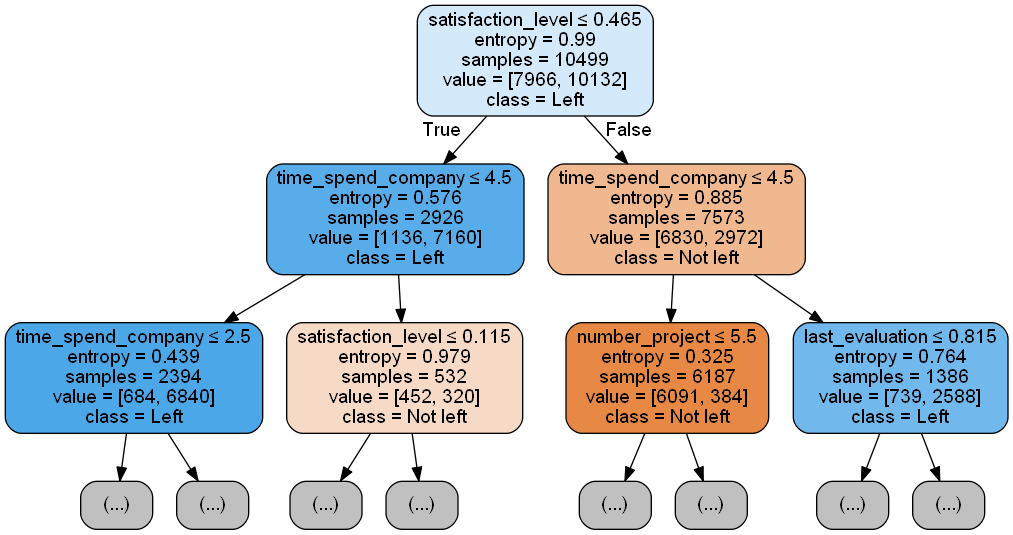
\includegraphics[width=\textwidth]{albero3}
    \captionof{figure}{Rappresentazione grafica del modello}
  \end{minipage}
  \hfill
  \begin{minipage}[b]{0.3\textwidth}
    \centering
    \setlength{\tabcolsep}{10pt} % Default value: 6pt
\renewcommand{\arraystretch}{1.5} % Default value: 1
\rowcolors{1}{grigio_chiaro}{white}
    \begin{tabularx}{\textwidth}{|lX|}
	\hline
	criterion                & entropy      \\
	max\_depth               & 3         \\
	min\_samples\_split      & 10         \\
	min\_samples\_leaf       & 10         \\
	class\_weight            & not left=1, left=4     \\\hline
	\end{tabularx}
      \captionof{table}{Parametri del modello}
      \label{img:model2}
    \end{minipage}
  \end{minipage}
  
\subsubsection*{Modello 3}
  
Anche in questo modello sono stati attribuiti pesi diversi alle due classi. Tuttavia, il vincolo sulla profondità massima è stato eliminato a favore di una strategia di \textit{pre-pruning} (alti valori di \texttt{min_samples_split} e \texttt{min_samples_leaf}).
Come nei modelli precedenti modelli, la prima suddivisione del modello in figura \ref{img:model3} riguarda \texttt{satisfaction_level}: 
\begin{itemize}
\item \texttt{satisfaction_level} $\leq$ 0.465: all'impiegato è assegnata la classe \texttt{Left}
\item \texttt{satisfaction_level} $>$ 0.465: un'ulteriore suddivisione viene effettuata in base al valore di \texttt{time_spend_company}. Se l'impiegato ha un valore dell'attributo superiore a 3.5, allora viene classificato come appartenente alla classe \texttt{Left}. In caso contrario, è molto probabile che ad egli venga attribuita l'etichetta \texttt{Not left} (divisione successiva: \texttt{average_montly_hours})
\end{itemize}\bigskip
  
\noindent \begin{minipage}{\textwidth}

  \begin{minipage}[b]{0.60\textwidth}
    \centering

    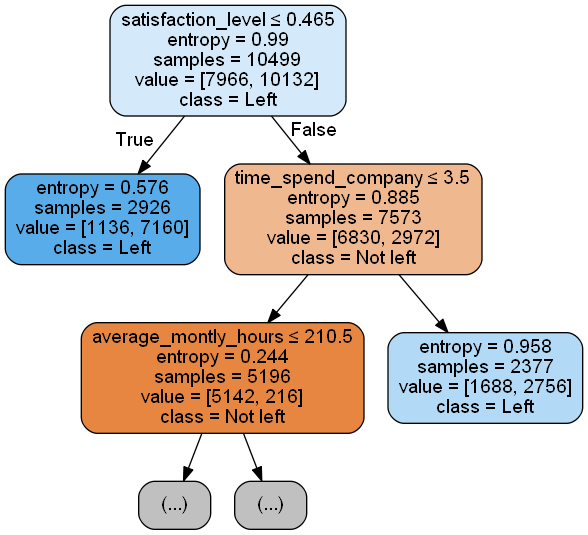
\includegraphics[width=0.85\textwidth]{albero2_bis}
    \captionof{figure}{Rappresentazione grafica del modello}

  \end{minipage}
  \hfill
  \begin{minipage}[b]{0.3\textwidth}
    \centering
    \setlength{\tabcolsep}{10pt} % Default value: 6pt
\renewcommand{\arraystretch}{1.5} % Default value: 1
\rowcolors{1}{grigio_chiaro}{white}
    \begin{tabularx}{\textwidth}{|lX|}
	\hline
	criterion                & entropy      \\
	max\_depth               & None         \\
	min\_samples\_split      & 200         \\
	min\_samples\_leaf       & 2000         \\
	class\_weight            & not left=1, left=4     \\\hline
	\end{tabularx}
      \captionof{table}{Parametri del modello}
      	    \label{img:model3}  
    \end{minipage}
  \end{minipage}
  
\subsubsection*{Modello 4}
L'unico vincolo di questo modello, seppur non molto stringente, riguarda \texttt{min_samples_split} e \texttt{min_samples_leaf}. Con un valore di 10 per entrambi i parametri, infatti, questa limitazione è apprezzabile soltanto ai livelli più bassi dell'albero.
Nel modello in figura \ref{img:model4}, ancora una volta, la prima suddivisione riguarda \texttt{satisfaction_level}: 
\begin{itemize}
\item \texttt{satisfaction_level} $\leq$ 0.465: se il valore di \texttt{time_spend_company} è minore o uguale a 4.5, l'etichetta assegnata con più probabilità è \texttt{Left} (con la divisione successiva di nuovo su \texttt{time_spend_company}). Se \texttt{time_spend_company} è invece maggiore di 4.5, il modello tende ad assegnare l'etichetta \texttt{Not left} (divisione successiva: \texttt{satisfaction_level})

\item \texttt{satisfaction_level} $>$ 0.465: come prima, suddividiamo in base a \texttt{time_spend_company}. Se l'impiegato ha un valore dell'attributo superiore a 4.5, allora tende ad essere classificato come appartenente alla classe \texttt{Left} (divisione successiva: \texttt{last_evaluation}). In caso contrario, è molto probabile che ad egli venga attribuita l'etichetta \texttt{Not left} (divisione successiva: \texttt{average_montly_hours})
\end{itemize}\bigskip
\noindent \begin{minipage}{\textwidth}

  \begin{minipage}[b]{0.65\textwidth}
    \centering

    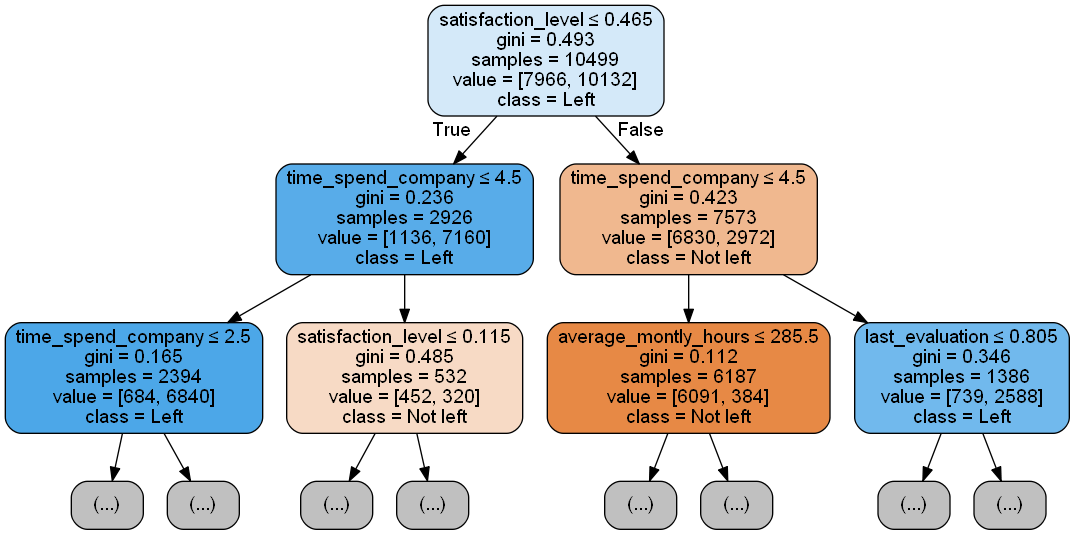
\includegraphics[width=\textwidth]{albero1}
    \captionof{figure}{Rappresentazione grafica del modello}
  \end{minipage}
  \hfill
  \begin{minipage}[b]{0.3\textwidth}
    \centering
    \setlength{\tabcolsep}{10pt} % Default value: 6pt
\renewcommand{\arraystretch}{1.5} % Default value: 1
\rowcolors{1}{grigio_chiaro}{white}
    \begin{tabularx}{\textwidth}{|lX|}
	\hline
	criterion                & gini      \\
	max\_depth               & None         \\
	min\_samples\_split      & 10         \\
	min\_samples\_leaf       & 10         \\
	class\_weight            & not left=1, left=4     \\\hline
	\end{tabularx}
      \captionof{table}{Parametri del modello}
          \label{img:model4}
    \end{minipage}
  \end{minipage}

\subsection{Validazione dei modelli}

In questa sezione si illustrano le performance dei modelli presentati nella sezione precedente. A questo scopo, il dataset originale è stato partizionato in \textit{Traning set} (70\%) e \textit{Test set} (30\%), utilizzando la tecnica del campionamento stratificato. Ogni modello è stato testato sui medesimi dati. Nella tabella \ref{tab:performances} sono mostrati i risultati: \newline

\begin{table}[h]
\centering
\begingroup
\setlength{\tabcolsep}{10pt} % Default value: 6pt
\renewcommand{\arraystretch}{1.5} % Default value: 1
\rowcolors{1}{grigio_chiaro}{white}

\begin{tabularx}{\textwidth}{|l|XXXX|XXXX|}
\hline
          & \multicolumn{4}{c|}{\textbf{Training set}} & \multicolumn{4}{c|}{\textbf{Test set}} \\
          & precision  & recall  & f1     & accuracy  & precision & recall & f1    & accuracy \\
Modello 1 & 0.851      & 0.847   & 0.826  & 0.847     & 0.861     & 0.857  & 0.838 & 0.857    \\
Modello 2 & 0.926      & 0.914   & 0.917  & 0.914     & 0.922     & 0.908  & 0.911 & 0.908    \\
Modello 3 & 0.864      & 0.726   & 0.745  & 0.726     & 0.868     & 0.723  & 0.745 & 0.723    \\
Modello 4 & 0.973      & 0.971   & 0.972  & 0.971     & 0.962     & 0.960  & 0.961 & 0.960   \\\hline
\end{tabularx}
\endgroup
\caption{Performance dei modelli}
\label{tab:performances}
\end{table}

\noindent La figura \ref{fig:confusions} mostra le diverse matrici di confusione dei modelli. Ognuna di esse mostra il numero dei \textit{True negative} (in alto a sx), dei \textit{False positive} (in alto a dx), dei \textit{False negative} (in basso a sx) e infine dei \textit{True positive} (in basso a dx).

\begin{figure}[h]
\centering
\begin{subfigure}[b]{.45\linewidth}
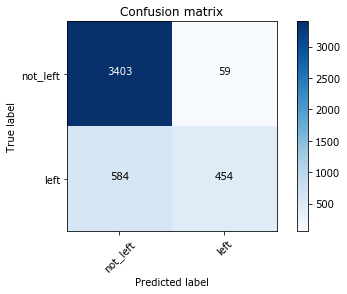
\includegraphics[width=\linewidth]{modello1Conf}
\caption{Matrice di confusione del modello 1}\label{subfig:conf1}
\end{subfigure}
\begin{subfigure}[b]{.45\linewidth}
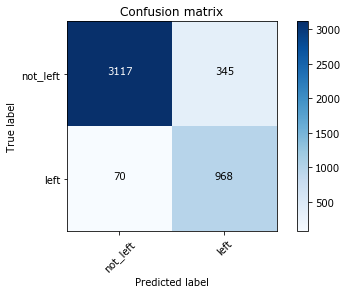
\includegraphics[width=\linewidth]{modello2Conf}
\caption{Matrice di confusione del modello 2}\label{subfig:conf2}
\end{subfigure}
\begin{subfigure}[b]{.45\linewidth}
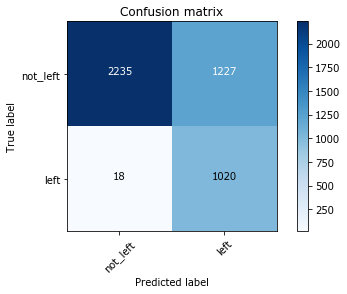
\includegraphics[width=\linewidth]{modello3Conf}
\caption{Matrice di confusione del modello 3}\label{subfig:conf3}
\end{subfigure}
\begin{subfigure}[b]{.45\linewidth}
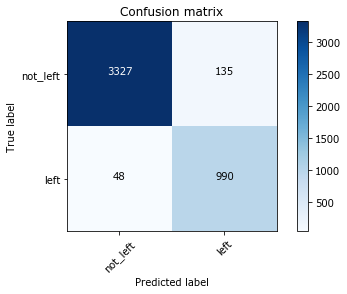
\includegraphics[width=\linewidth]{modello4Conf}
\caption{Matrice di confusione del modello 4}\label{subfig:conf4}
\end{subfigure}
\caption{Matrici di confusione dei modelli}
\label{fig:confusions}
\end{figure}

\subsection{Identificazione del miglior modello}

Per la ricerca del miglior modello \textit{M} (dal punto di vista delle performance) è stato utilizzata strategia basata su \textit{Random Forest}. Questa soluzione consiste nel creare diversi alberi di decisione (ognuno dei quali è allenato su diversi sottoinsiemi del dataset usato per la fase di \textit{training}). Le decisioni prese da questo modello dipendono dalle decisioni prese dai singoli alberi: in questo caso, la decisione presa dalla \textit{Random Forest} è la decisione presa dalla maggior parte degli alberi della foresta (moda).

La scelta dei migliori parametri da utilizzare per il modello \textit{M} è stata approssimata utilizzando una tecnica di \textit{Grid search} con ricerca casuale. Tra tutte le possibili combinazioni di parametri illustrate nella tabella \ref{tab:gridParams} (fornite tramite specifici intervalli di valori) sono state scelte casualmente 100 configurazioni e, tra di esse, è stata selezionata la migliore (vedere ancora la tabella \ref{tab:gridParams}). La funzione scelta per la misurazione della qualità delle suddivisioni è l'\textit{Information Gain} (basata sull'\texttt{entropy}). Per la massima profondità dell'albero, invece, è stato scelto il valore 9: intuitivamente, un valore più alto avrebbe prodotto un modello con problemi di \textit{Overfitting}. Sia per \texttt{min_samples_split} che per \texttt{min_samples_leaf} sono stati scelti due valori molto bassi: in altre parole, si è ritenuto più vantaggioso non usare tecniche di \textit{Pre-pruning}. 
Parlando invece dei pesi assegnati alle classi \texttt{not_left} e \texttt{left}, notiamo che l'opzione ritenuta più efficiente è assegnare ad entrambe le classi lo stesso peso (valore \texttt{None}).


Infine, la tabella \ref{tab:performancesOfBestModel} illustra le performance di \textit{M} su \textit{Training set} e \textit{Test set}. L'albero di decisione corrispondente è riportato nella figura \ref{fig:best_model_representation}: analogamente agli altri modelli studiati nella precedente sezione, vediamo che la prima suddivisione dei record avviene sull'attributo \texttt{satisfaction_level}. Al primo livello dell'albero, le suddivisioni si basano unicamente sull'attributo \texttt{number_project}: ad eccezione del modello 1 (figura \ref{img:model1}), nessuno degli altri modelli aveva utilizzato questa feature nelle decisioni del primo livello. Riguardo a \texttt{Work_accident}, invece, il modello \textit{M} è l'unico ad averlo coinvolto nelle decisioni dei primi due livelli. 


La figura \ref{fig:feat_imp_best_mod} mostra invece l'importanza di ogni attributo nel processo di decisione di \textit{M}: in accordo con la prima suddivisione nella rappresentazione grafica dell'albero, vediamo che \texttt{satisfaction_level} è la feature che più incide nel processo di decisione. Seguono poi \texttt{time_spend_company} e \texttt{number_project}, mentre è evidente la poca influenza delle feature \texttt{salary} e \texttt{Work_accident}.\newline

Allo scopo di attuare un confronto generale tra tutti i modelli precedentemente illustrati, la figura \ref{fig:roc_curves_all_models} mostra le curve ROC per tutti i modelli analizzati in precedenza.



\begin{table}[h]

\begin{minipage}[b]{0.4\textwidth}

\centering
\setlength{\tabcolsep}{10pt} % Default value: 6pt
\renewcommand{\arraystretch}{1.5} % Default value: 1
\rowcolors{1}{grigio_chiaro}{white}
    \begin{tabularx}{\textwidth}{|XXX|}
	\hline
	\textbf{Parametro}       & \textbf{Intervallo}  & \textbf{Valore scelto} \\
	criterion                & ['gini', 'entropy']  & entropy   \\
	max\_depth               & [None]  & 9       \\
	min\_samples \_split      & [2, 3, ..., 51] & 8         \\
	min\_samples \_leaf       & [2, 3, ..., 51] & 2        \\
	class\_weight            & [(not\_left=1, left=4), None, Balanced]   & None  \\\hline
	\end{tabularx}
      \captionof{table}{Griglia dei parametri del modello \textit{M} e valori selezionati}
          \label{tab:gridParams}

\end{minipage}
\hfill
\begin{minipage}[b]{0.55\textwidth}
\centering

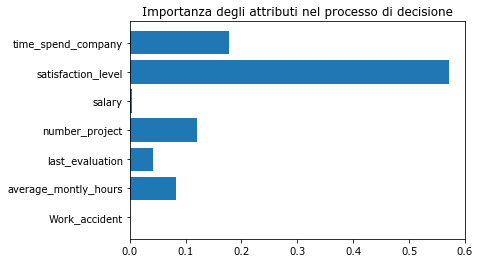
\includegraphics[width=\textwidth]{feat_imp_best_model}
\captionof{figure}{Feature importance del modello \textit{M}}
\label{fig:feat_imp_best_mod}
\end{minipage}

\end{table}

\begin{table}[h]
\centering
\begingroup
\setlength{\tabcolsep}{10pt} % Default value: 6pt
\renewcommand{\arraystretch}{1.5} % Default value: 1
\rowcolors{1}{grigio_chiaro}{white}

\begin{tabularx}{\textwidth}{|XXXX|XXXX|}
\hline
          \multicolumn{4}{|c|}{\textbf{Training set}} & \multicolumn{4}{c|}{\textbf{Test set}} \\
          precision  & recall  & f1     & accuracy  & precision & recall & f1    & accuracy \\
 0.983      & 0.983   & 0.983  & 0.983     & 0.974     & 0.974  & 0.974 & 0.974    \\
\hline
\end{tabularx}
\endgroup
\caption{Performance del modello \textit{M}}
\label{tab:performancesOfBestModel}
\end{table}

\begin{center}
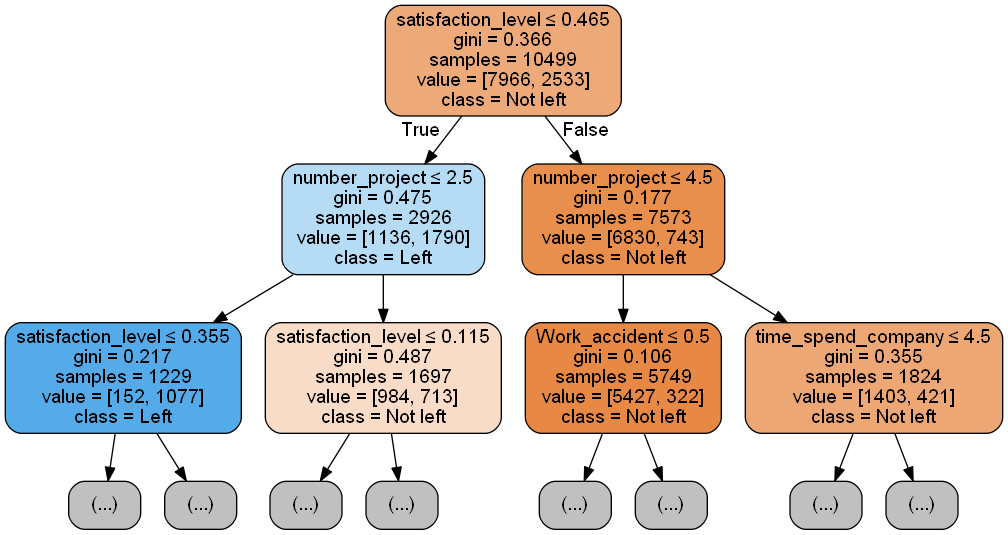
\includegraphics[width=0.7\textwidth]{best_model_representation}
\captionof{figure}{Rappresentazione grafica del modello \textit{M}}
\label{fig:best_model_representation}

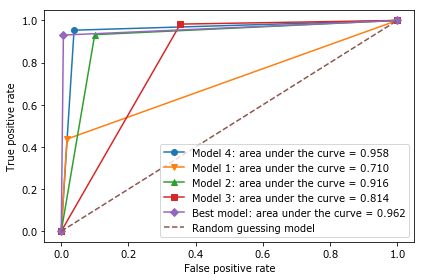
\includegraphics[width=0.5\textwidth]{roc_curves}
\captionof{figure}{Curve ROC dei modelli precedentemente analizzati}
\label{fig:roc_curves_all_models}

\end{center}

%\begin{minipage}{\textwidth}
%
%  \begin{minipage}[b]{0.65\textwidth}
%    \centering
%
%    
%  \end{minipage}
%  \hfill
%  \begin{minipage}[b]{0.3\textwidth}
%    \centering
%    
%    \end{minipage}
%  \end{minipage}

\end{document}
